\documentclass[conference,compsoc]{IEEEtran}
\usepackage{./macros}

\begin{document}
\vspace{3cm}
\title{CS5610 Assignment 1}
\author{Gautam Singh\\CS21BTECH11018}
\maketitle
\tableofcontents

\bigskip

\begin{abstract}
    This report analyzes the various techniques implemented for a multi-threaded
    solution to computing the sparsity of a matrix. The sparsity of a matrix is
    defined as the number of zero entries in the matrix. The report is organized
    as follows. In \autoref{sec:block-dynamic}, we introduce a new technique to
    compute sparsity. Then, we provide a low-level overview of the C++
    implementation. In \autoref{sec:prog-design}, we describe the low-level
    program design on which our experiments are run. In \autoref{sec:results},
    we present the results of various experiments and analyze them. Finally, we
    conclude the report in \autoref{sec:conclusion}.  
\end{abstract}

\section{Dynamic Block Allocation}
\label{sec:block-dynamic}

In this section, we describe a new technique to compute the sparsity of a square
matrix. In this method, we divide the matrix into square blocks of size \(M\),
for a total of \(\brak{\ceil{\frac{N}{M}}}^2\) blocks. Each thread gets a block
and computes the sparsity of a matrix by iterating through the elements in that
block.

To make this \emph{block allocation} technique dynamic in nature, we allocate
ids to each block in row-major order. Formally, if \(P = \ceil{\frac{N}{M}}\),
then the \(j\)-th block in the \(i\)-th row of blocks will be given the id \(Pi
+ j\), where \(i\) and \(j\) are zero-indexed. Therefore, to obtain blocks,
threads will increment a shared counter atomically until the limit on the number
of blocks (which is \(P^2\)) is reached.

Allocation of blocks attempts to exploit spatial as well as temporal locality of
the rows of the matrix to prevent cache misses.

\section{Program Design}
\label{sec:prog-design}

We describe the low-level program design of our C++ implementation used to
compute the sparsity of the input matrix.

\subsection{Command Line Options}
\label{subsec:cmd-line-options}

The program takes various arguments that can be found in the \texttt{help}
function of the code. In particular, the technique to be used is specified using
the command line and parsed during execution. Runner functions for each
technique have been implemented. Based on the chosen technique, all threads run
one of the implemented functions to compute the sparsity of the matrix.

\subsection{Threads and Thread Information}
\label{subsec:threads}

All of the runner functions receive a \texttt{ThreadInfo} struct which is
defined as follows.

\begin{listing}[!ht]
\inputminted{cpp}{codes/ThreadInfo.cpp}
\caption{The ThreadInfo struct.}
\label{code:ThreadInfo}
\end{listing}

On executing the runner function, the sparsity computed by this thread is stored
in the field \texttt{res}. For static methods, the \texttt{id} field is used to
compute the allocation of rows to this thread. Since thread ids assigned by the
operating system may not be in the range \([0, N)\), we assign our own thread
ids for use.

Threads are created using the \texttt{thread} class in the C++ standard library.
Based on the technique to be used, they are instantiated with the runner
function and their corresponding \texttt{ThreadInfo} struct that contains all
the necessary information.

\subsection{Atomic Shared Counters}
\label{subsec:counter}

For dynamic methods, such as the dynamic row and block allocation techniques, we
create a \texttt{Counter} class, whose memebers and methods are defined as
follows. Full implementation details can be found in the source code, and are
omitted for brevity.

\begin{listing}[!ht]
\inputminted{cpp}{codes/Counter.cpp}
\caption{The \texttt{Counter} class.}
\label{code:Counter}
\end{listing}

The \texttt{Counter} class is a template class, meaning one can instantiate a
counter using integral data-types of various sizes and signedness. For our
purposes, we use a 64-bit unsigned integer as the integral data type. The atomic
operations are provided by the \texttt{atomic} class in the C++ standard
library. The following methods are implemented:

\begin{enumerate}
    \item \texttt{T get()}: Read the current value stored in the counter
    atomically. Threads use this to check how many rows or blocks have their
    sparsity computed.
    \item \texttt{T getAndIncrement(T inc)}: Read the current value and then
    increment the counter by \texttt{inc}. Threads use this to get the id of the
    row or block on which sparsity is to be computed. 
\end{enumerate}

\subsection{Timing}
\label{sec:timing}

The \texttt{chrono} class provided by the C++ library was used to measure
execution time. Specifically, the time taken from creation of threads to their
joining was measured in milliseconds. 

\section{Results and Analysis}
\label{sec:results-and-analysis}

The following experiments have been performed on an Intel i9-11900H 8-core
16-thread CPU. We analyze the variation of execution time on varying different
parameters one-by-one. Note that the variable \texttt{rowInc} is taken as block
increment for the dynamic block allocation method.

\subsection{Time vs. Size}
\label{subsec:time-vs-size}

\begin{figure}[!ht]
    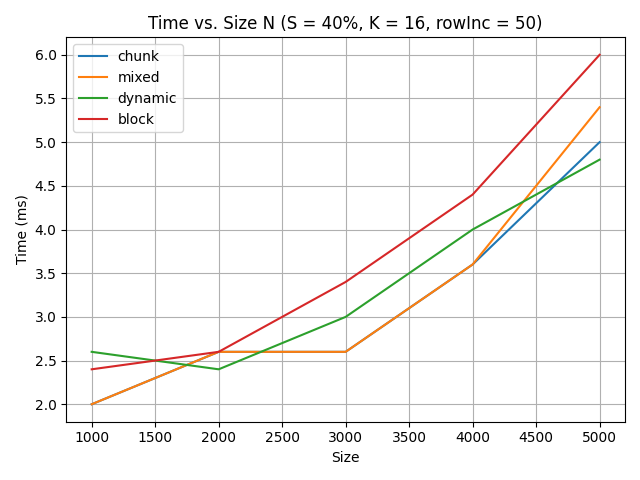
\includegraphics[width=\columnwidth]{images/exp1.png}
    \caption{Execution time vs. matrix size for various techniques.}
    \label{fig:exp-1}
\end{figure}

\autoref{fig:exp-1} shows the execution time for various methods as matrix size
\(N\) changes. We set the number of threads \(K = 16\), row increment \(rowInc =
50\) and sparsity \(S = 40\%\). The total number of zero elements is shown in
\autoref{tab:exp1-table}. We observe the following.

\begin{table}[!ht]
    \begin{tabularx}{\columnwidth}{|Y|Y|Y|Y|Y|Y|}
        \hline
        \textbf{Size \(N\)} & 1000 & 2000 & 3000 & 4000 & 5000 \\
        \hline
        \textbf{No. of Zeros (\(\times 10^6\))} & 0.4 & 1.6 & 3.6 & 6.4 & 10 \\
        \hline
    \end{tabularx}
    \caption{Number of zeros for 40\% sparsity as a function of matrix size.}
    \label{tab:exp1-table}
\end{table}

\begin{enumerate}
    \item Execution time for all methods increases with size quadratically.
    \item Dynamic row allocation performs the best but dynamic block allocation
    performs the worst. However, the time difference is within 1.5 ms for all
    methods for a matrix of size 5000.
\end{enumerate}

\subsection{Time vs. Number of Threads}
\label{subsec:exp2}

\begin{figure}[!ht]
    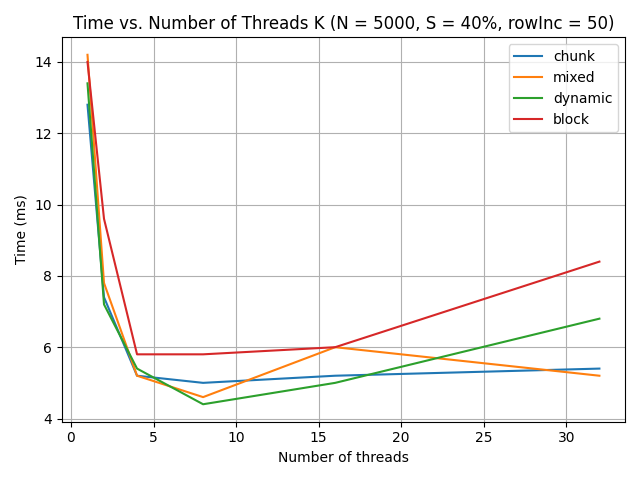
\includegraphics[width=\columnwidth]{images/exp2.png}
    \caption{Execution time vs. number of threads for various techniques.}
    \label{fig:exp-2}
\end{figure}

\autoref{fig:exp-2} shows the execution time for various methods as the number
of threads increases. We set \(N = 5000\), \(S = 40\%\) and \(rowInc = 50\). The
following observations can be made.

\begin{enumerate}
    \item The best performance occurs when using 8 threads. As the number of
    threads increases, initially the execution time reduces drastically.
    However, on still increasing the number of threads, the delay during context
    switches dominates, thus the total execution time increases.
    \item The static allocation methods outperform the dynamic allocation
    methods, since less work is given to each thread. In fact, the execution
    times level out for both static methods.
    \item The larger execution times for the dynamic methods may also be due to
    competition for incrementing the shared atomic counter.
\end{enumerate}

\subsection{Time vs. Sparsity}
\label{subsec:exp3}

\begin{figure}[!ht]
    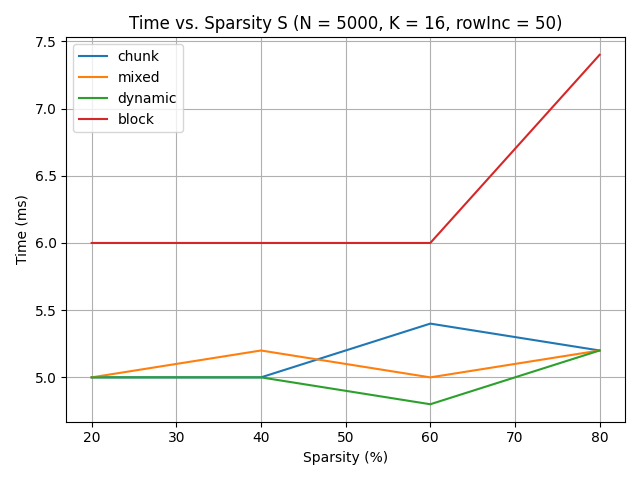
\includegraphics[width=\columnwidth]{images/exp3.png}
    \caption{Execution time vs. sparsity for various techniques.}
    \label{fig:exp-3}
\end{figure}

\autoref{fig:exp-3} shows the execution time for various methods as the sparsity
of the matrix increases. We set \(N = 5000\), \(K = 16\) and \(rowInc = 50\).
The number of zeros computed in each case are depicted in
\autoref{tab:exp3-table}. The following observations can be made.

\begin{table}[!ht]
    \begin{tabularx}{\columnwidth}{|Y|Y|Y|Y|Y|}
        \hline
        \textbf{Sparsity} & 20\% & 40\% & 60\% & 80\% \\
        \hline
        \textbf{No. of Zeros (\(\times 10^6\))} & 5 & 10 & 15 & 20 \\
        \hline
    \end{tabularx}
    \caption{Number of zeros for various sparsity levels where \(N = 5000\).}
    \label{tab:exp3-table}
\end{table}

\begin{enumerate}
    \item Except for the block method, other techniques are more or less at the
    same performance despite an increase in sparsity.
    \item For the block method, the larger execution times are a result of
    threads having to compete for incrementing the shared counter, as well as
    doing the extra work of decoding the location of the block from the block id
    provided by the shared counter. This results in a slower execution by about
    2 milliseconds.
\end{enumerate}

\subsection{Time vs. Row Increment}
\label{subsec:exp4}

\begin{figure}[!ht]
    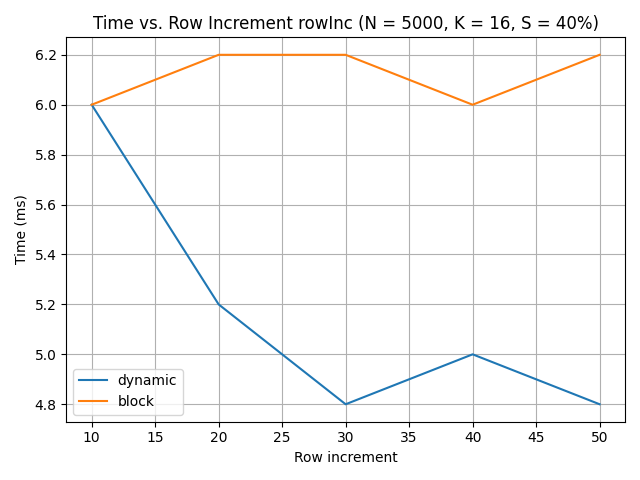
\includegraphics[width=\columnwidth]{images/exp4.png}
    \caption{Execution time vs. Row increments for dynamic allocation methods.}
    \label{fig:exp-4}
\end{figure}

\autoref{fig:exp-4} shows the execution time for various dynamic methods as the
row increments change. We set \(N = 5000\), \(S = 40\%\) and \(K = 16\). The
following observations can be made.

\begin{enumerate}
    \item The execution time for dynamic block allocation remains the same on
    increasing the block increment, whereas it decreases for dynamic row
    allocation.
    \item In a dynamic setting, row allocation beats block allocation, by 1.4
    milliseconds on average. Threads have less decoding to do from the shared
    counter during dynamic row allocation, which explains the speedup.
\end{enumerate}

\section{Conclusion}
\label{sec:conclusion}

We conclude that both chunk and mixed methods give very good performance as the
number of threads increases. However, dynamic row allocation is better with a
lesser number of threads. Because of the excessive decoding work in this
implementation, dynamic block allocation did not perform as well as dynamic row
allocation on increasing the size of the matrix and also on increasing sparsity.
Therefore, one should consider allocation methods and techniques that have very
little overhead.

\end{document}